%%%%%%%%%%%%%%%%%%%%%%%%%%%%%%%%%%%%%%%%%%%%%%%%%%%%%%%%%%%%%%%%%%%%%%%%%%%%%%%%%%
\begin{frame}[fragile]\frametitle{}
\begin{center}
{\Large Conclusions}
\end{center}
\end{frame}

%%%%%%%%%%%%%%%%%%%%%%%%%%%%%%%%%%%%%%%%%%%%%%%%%%%%%%%%%%%
\begin{frame}[fragile]\frametitle{In General}
  \begin{itemize}
    \item Autonomous AI Agents powered by Large Language Models represent AI pinnacle.
    \item Abilities in planning, memory utilization, and tool use, combined with a flawless workflow, open exciting possibilities across industries.
    \item A future where AI-driven efficiency and problem-solving reach unprecedented heights.
    \item Machines that think, remember, and adapt — a revolution in AI.
  \end{itemize}
\end{frame}


%%%%%%%%%%%%%%%%%%%%%%%%%%%%%%%%%%%%%%%%%%%%%%%%%%%%%%%%%%%%%%%%%%%%%%%%%%%%%%%%%%
\begin{frame}[fragile]\frametitle{Challenges in LLM-Centered Agents}
  \begin{itemize}

    \item Finite Context Length: Restricted context capacity limits inclusion of historical information, detailed instructions, API call context, and responses.
    % \item System design works with limited communication bandwidth, impacting mechanisms like self-reflection.
    \item Long-term planning and task decomposition: LLMs struggle to adjust plans when faced with unexpected errors.
    % \item Planning over lengthy history and exploring solution space remain challenging for LLMs.
    \item Less robust compared to humans who learn from trial and error.
    % \item Reliability of Natural Language Interface: Current agent system relies on natural language as an interface, but the reliability of model outputs is questionable.
    \item LLMs may make formatting errors and occasionally exhibit rebellious behavior (e.g., refuse to follow an instruction).
    % \item Agent demo code often focuses on parsing model output due to these reliability issues.
  \end{itemize}
\end{frame}

%%%%%%%%%%%%%%%%%%%%%%%%%%%%%%%%%%%%%%%%%%%%%%%%%%%%%%%%%%%%%%%%%%%%%%%%%%%%%%%%%%
\begin{frame}[fragile]\frametitle{When to Use Agents}
\begin{itemize}
    \item Ideal for tasks requiring \textbf{complex decision-making}, \textbf{autonomy}, and \textbf{adaptability}.
    \item Useful in \textbf{dynamic workflows} with multiple steps and automation potential.
    \item \textbf{Customer support}: Handle queries, provide real-time assistance, and escalate issues.
    \item Enhances \textbf{efficiency} and \textbf{customer experience} with timely responses.
    \item \textbf{Research and data analysis}: Autonomously gather, process, and analyze data.
    \item Suitable for \textbf{real-time data processing} like financial trading.
    \item Beneficial in \textbf{education}: Personalized learning, adaptive pacing, and instant feedback.
    \item \textbf{Software development}: Assist in code generation, debugging, and testing.
    \item Agents improve through \textbf{learning and adaptation}, crucial for continuous improvement.
\end{itemize}
\end{frame}

%%%%%%%%%%%%%%%%%%%%%%%%%%%%%%%%%%%%%%%%%%%%%%%%%%%%%%%%%%%%%%%%%%%%%%%%%%%%%%%%%%
\begin{frame}[fragile]\frametitle{When Not to Use Agents}
\begin{itemize}
    \item Avoid for \textbf{straightforward or infrequent tasks} requiring minimal automation.
    \item Traditional methods are more \textbf{efficient and cost-effective} for simple tasks.
    \item Unsuitable for tasks needing \textbf{deep domain-specific expertise} or complex knowledge.
    \item Examples: Legal analysis, medical diagnoses, or high-stakes decisions in uncertain contexts.
    \item Not ideal for tasks requiring \textbf{empathy, creativity, or subjective judgment}.
    \item Examples: Psychotherapy, counseling, or creative writing.
    \item Implementation demands \textbf{time, resources, and expertise}.
    \item May not be viable for \textbf{small businesses or limited budgets}.
    \item Challenges in \textbf{highly regulated industries}: Compliance and security concerns.
    \item Ensuring adherence to \textbf{regulatory requirements} can be resource-intensive.
\end{itemize}
\end{frame}


%%%%%%%%%%%%%%%%%%%%%%%%%%%%%%%%%%%%%%%%%%%%%%%%%%%%%%%%%%%%%%%%%%%%%%%%%%%%%%%%%%
\begin{frame}[fragile]\frametitle{Are you creative enough?}
		\begin{center}
		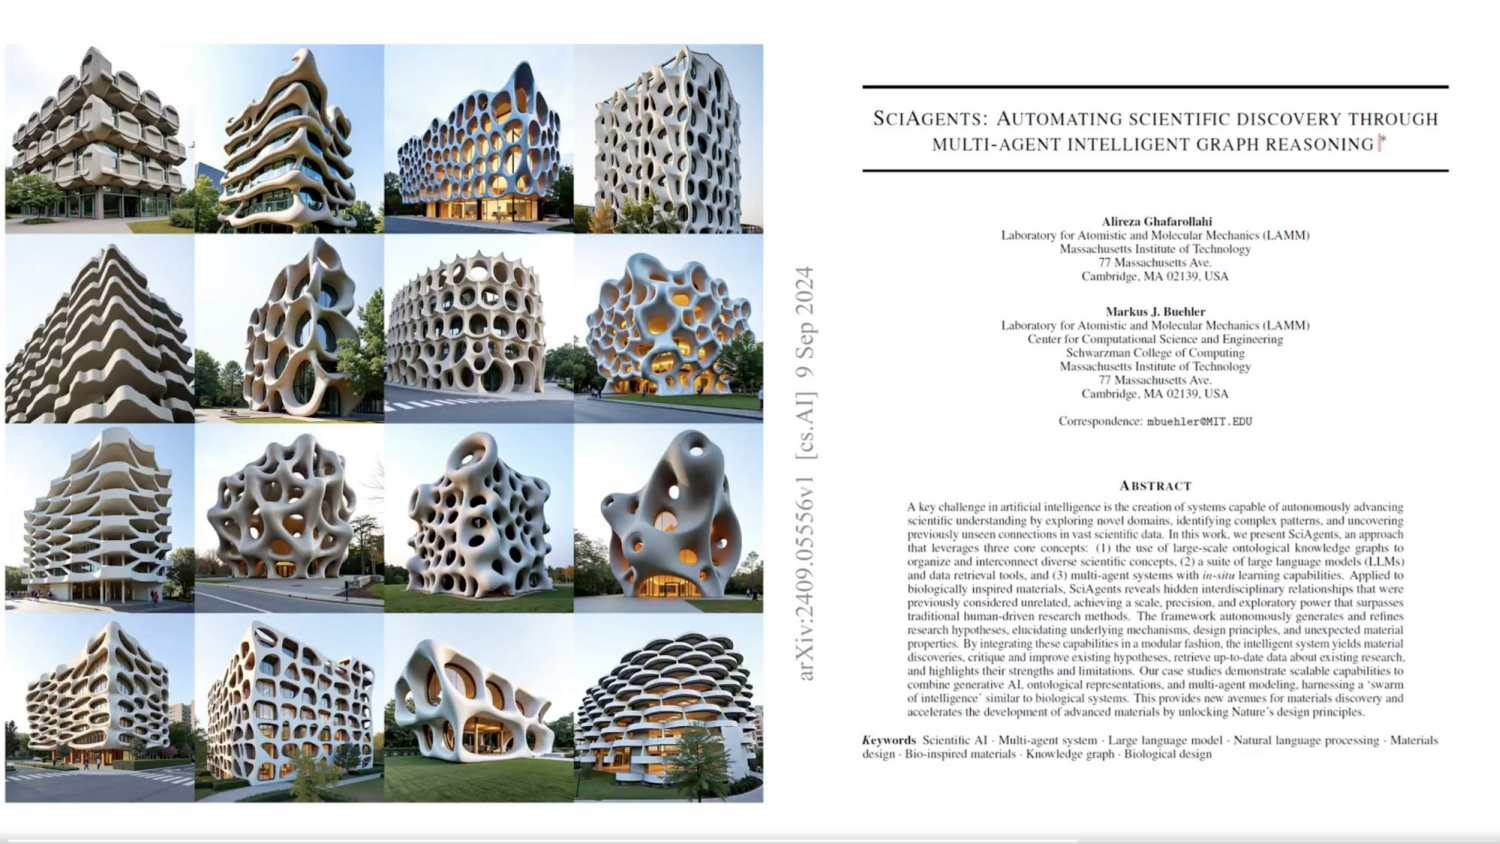
\includegraphics[width=\linewidth,keepaspectratio]{autoagent8}
		\end{center}
		
		{\tiny (Ref: Agentic AI Frameworks \& AutoGen - Chi Wang)}
\end{frame}
  

%%%%%%%%%%%%%%%%%%%%%%%%%%%%%%%%%%%%%%%%%%%%%%%%%%%%%%%%%%%
\begin{frame}[fragile]\frametitle{My Sketchnote}
	
	\begin{center}
	\includegraphics[width=0.45\linewidth,keepaspectratio]{AutonomousAIAgents_Sketchnote}
	\end{center}
{\tiny (Ref: Power of Autonomous AI Agents - Yogesh Kulkarni)}
\end{frame}

%%%%%%%%%%%%%%%%%%%%%%%%%%%%%%%%%%%%%%%%%%%%%%%%%%%%%%%%%%%
\begin{frame}[fragile]\frametitle{The Future with AutoGen}
  \begin{itemize}
    \item Transformative era in AI collaboration is on the horizon.
    \item Microsoft’s vision for Autonomous AI Agents and AutoGen's capabilities provide a glimpse into the future of AI applications.
    % \item Collaboration, innovation, and democratization are at the core of AutoGen’s mission.
    \item Empowers professionals to navigate the complex AI landscape with confidence, agility, and precision.
    % \item The journey has just begun, and the possibilities with AutoGen are endless.
  \end{itemize}
\end{frame}

%%%%%%%%%%%%%%%%%%%%%%%%%%%%%%%%%%%%%%%%%%%%%%%%%%%%%%%%%%%
\begin{frame}[fragile]\frametitle{Towards Artificial General Intelligence (AGI)}
  \begin{itemize}
    \item Research aligns with the belief that achieving human-like general intelligence requires cooperation among agents.
    \item Multi-agent collaboration is a crucial approach, but it may not alone pave the path to artificial general intelligence (AGI).
    \item The journey likely demands additional innovations and breakthroughs.
	\item AutoGen stands out as an enticing platform for exploring possibilities offered by multi-agent systems.
  \end{itemize}
\end{frame}
